\documentclass{article}
\usepackage[utf8]{inputenc}
\usepackage[T1]{fontenc}
\usepackage[portuguese]{babel}

\usepackage{indentfirst}
\usepackage{makeidx}
\usepackage{stackengine}
\usepackage{amssymb}
\usepackage{amsthm}
\usepackage{hyperref}
\usepackage{color}
\usepackage{graphicx}

\usepackage{booktabs}

\title{\bf{Aprendizagem Computacional - Trabalho Prático 3}\vspace{80mm}}
\author{\textbf{João Tiago Márcia do Nascimento Fernandes - 2011162899} \\
\textbf{Joaquim Pedro Bento Gonçalves Pratas Leitão - 2011150072}}
\makeindex

\begin{document}

\maketitle

\pagebreak

\renewcommand*\contentsname{Índice}
\tableofcontents

\pagebreak

\section{Introdução}

O presente trabalho foca-se na previsão e identificação de crises epiléticas, com base em informação de sinais cerebrais, recolhidos através da realização de um \emph{EEG} (ElectroEncefaloGrama).

Este exame recolhe dados relativos à atividade cerebral do paciente que o realiza, sendo possível extrair um conjunto de características que permite a identificação de momentos de ocorrência de crises epiléticas (situações \emph{ictais}) e de momentos nos quais o paciente não apresenta qualquer problema (situações \emph{não-ictais}).

O trabalho proposto visa a criação de uma aplicação em \emph{Matlab}, que analise os dados recolhidos após a realização de um \emph{EEG} a um paciente, e que identifique eventuais situações em que a atividade cerebral registada corresponde a uma situação de crise epilética.

Para proceder à identificação das situações \emph{ictais} e \emph{não-ictais}, a aplicação desenvolvida faz uso, na sua arquitetura interna, de redes neuronais, disponíveis na \emph{Neural Networks Toolbox} do próprio \emph{Matlab}.

Para avaliar o desempenho e performance da aplicação desenvolvida, procederemos à análise da sensibilidade e especificidade de cada rede neuronal implementada.

Estas métricas correspondem à percentagem de situações \emph{ictais} verdadeiras detetadas (\emph{sensibilidade}) e à percentagem de situações \emph{não-ictais} falsas detetadas (\emph{especificidade}), refletindo a performance da rede na classificação de um dado \emph{data set}: Uma elevada \emph{sensibilidade} implica uma boa deteção de situações \emph{ictais}, enquanto que uma elevada \emph{especificidade} implica uma boa deteção de casos \emph{não-ictais}.

Ambas as métricas constituem requisitos necessários para a sua utilização em ambiente clínico, e podem ser definidas da seguinte forma:

$$Sensibilidade \: = \frac{PositivosVerdadeiros}{PositivosVerdadeiros + FalsosNegativos}$$

$$Especificidade \: = \frac{NegativosVerdadeiros}{NegativosVerdadeiros + FalsosPositivos}$$

\vspace{.1cm}

No presente documento pretendemos apresentar de forma mais detalhada a aplicação desenvolvida, discutindo alguns detalhes da sua implementação e apresentando uma reflexão crítica sobre o seu desempenho e performance, nomeadamente da sua sensibilidade e especificidade.

\pagebreak

\section{Aplicação Desenvolvida}

Tal como referido anteriormente, a aplicação desenvolvida visa analisar os dados referentes a um \emph{EEG} de um paciente, identificando situações correspondentes a uma crise epilética.

Esta classificação pode ser realizada de duas formas distintas.

Numa primeira abordagem, a que chamamos \emph{Classificação Individual}, é atribuído a cada elemento do conjunto de dados de entrada da aplicação uma de duas \emph{classes}, representadas por dois valores binários:

\begin{itemize}
\item Classe \emph{não-ictal}, correspondente a um estado normal do paciente (ausência de crises) e representada pelos valores \emph{1 0}

\item Classe \emph{ictal}, correspondente a uma situação de crise, e representada pelos valores \emph{0 1}
\end{itemize}

Na segunda abordagem, a que chamamos \emph{Classificação em Grupo}, a classificação é realizada de forma semelhante, no entanto são considerados conjuntos de dados de entrada da aplicação, ao invés de cada elemento. Para este tipo de classificação podemos adotar duas métricas diferentes:

\begin{itemize}
\item Analisar o número de elementos consecutivos classificados individualmente como \emph{ictais}, comparando-o com um dado limiar. Neste caso, se, por exemplo, existirem pelo menos 10 elementos consecutivos classificados como \emph{ictais} então é detetada uma crise. Caso contrário nenhuma crise é detetada.

\item Adotar um sistema de classificação em janela deslizante, analisando o número de elementos classificados individualmente como \emph{ictias}, num dado universo restrito. Isto é, se pelo menos cinco dos últimos dez elementos foram classificados como \emph{ictais} então todos os elementos nesse conjunto são classificados como \emph{ictais}.
\end{itemize}

Relativamente a este último aspeto, optámos por adotar o segundo método de \emph{Classificação em Grupo}, considerando uma abordagem por janelas.

De seguida apresentamos em maior detalhe a aplicação desenvolvida, salientando alguns dos seus aspetos mais importantes e relevantes.

\subsection{Graphical User Interface}

Para facilitar a interação do utilizador com a aplicação, foi-nos proposta a criação de uma interface gráfica onde são solicitadas ao utilizador todas as informações relevantes para a execução da aplicação, separando por completo a sua lógica interna com a especificação dos seus dados de entrada e outros parâmetros.

Assim, na interface gráfica desenvolvida são solicitadas ao utilizador várias informações que permitem a criação e treino das diferentes redes neuronais, nomeadamente:

\begin{itemize}
\item Tipo de rede neuronal a criar e treinar. Encontram-se disponíveis as redes \emph{Radial Basis Function}, \emph{Layer Recurrent Network}, \emph{FeedForward}, \emph{FeedForward Time Input Delay} e \emph{Distributed Time Delay}.

\item Função de Aprendizagem (ou Função de Treino) a utilizar na rede neuronal a criar (Se necessário). Encontram-se disponíveis as funções \emph{trainscg}, \emph{traingd} e \emph{trainrp}.

\item Função de Performance a utilizar no treino da rede neuronal (se necessário). Estão disponíveis as funções \emph{mse} (mean squared error) e \emph{sse} (sum squared error).

\item Função de Activação dos neurónios da rede neuronal a implementar (se necessário). Estão disponíveis as funções \emph{hardlim}, \emph{purelin}, \emph{logsig} e \emph{tansig}.

\item Tipo de Classificação a realizar (\emph{Individual} ou \emph{Em Grupo})

\item Ficheiro de dados a utilizar para treinar a rede criada

\item Ficheiro de dados a utilizar para testar a rede criada

\item Outros aspetos, como objetivo do treino (\emph{Goal}), taxa de aprendizagem, etc
\end{itemize}

Para além disso, na interface desenvolvida, existe também uma secção onde são apresentados os resultados de cada teste realizado, nomeadamente a especificidade e sensibilidade da rede considera.

\begin{figure}[h]
  \centering
      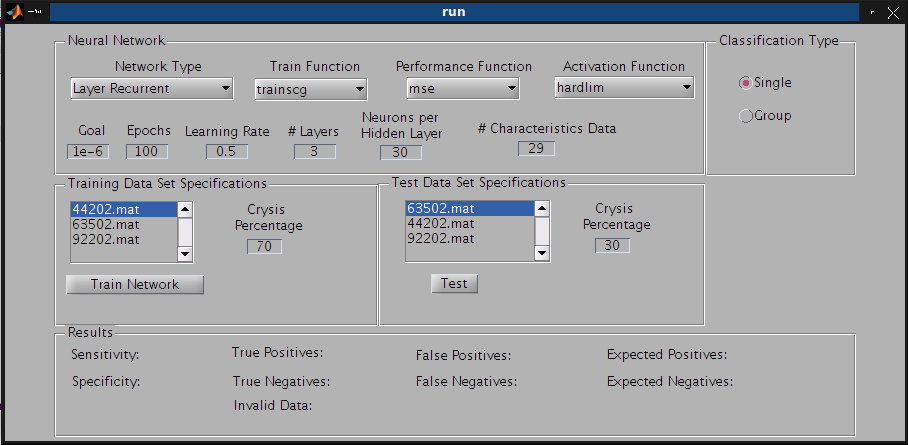
\includegraphics[scale=0.3]{Images/Aplication_GUI.png}
  \caption{Interface Gráfica implementada}
\end{figure}

\subsection{Redes Neuronais Implementadas}

Como já referimos anteriormente, na nossa aplicação implementámos cinco redes neuronais distintas: \emph{Radial Basis Function}, \emph{Layer Recurrent Network}, \emph{FeedForward}, \emph{FeedForward Time Input Delay} e \emph{Distributed Time Delay}.

Estas redes apresentam, naturalmente, características e propriedades distintas, sendo que umas se adequam mais ao trabalho que pretendemos realizar do que outras.

Por exemplo, considerando a rede \emph{Layer Recurrent}, esta rede permite a introdução de atrasos em algumas características, o que lhe permite aprender a prever qualquer saída dinâmica, tendo por base entradas passadas. Este processo é possível se forem considerados neurónios e atrasos suficientes na rede.

De facto, esta é uma propriedade que vai, de certa forma, ao encontro do funcionamento de um cérebro humano, que para além de ser um sistema dinâmico, possui também memória.

Na mesma linha de raciocínio, redes que suportam a introdução de atrasos em algumas das características que constituem os dados de entrada surgem, a uma primeira vista, como boas opções para simular o comportamento de um cérebro humano, realizando uma melhor identificação das situações correspondentes a crises epiléticas. Exemplos destas redes são a rede \emph{Distributed Time Delay} e a \emph{FeedForward Input Time Delay}.

Por seu turno, a rede \emph{FeedForward} também se apresenta como uma solução a considerar, dado o facto de permitir uma boa implementação de qualquer função de entradas e saídas arbitrárias, desde que considerados neurónios suficientes na(s) camada(s) escondida(s).

Por fim, é também necessário referir a rede \emph{Radial Basis Function}, bastante utilizada para aproximar funções e cujo treino passa nomeadamente pela adição de neurónios à camada escondida até que a rede atinja a performance (\emph{goal}) pretendida. Assim, embora possa ser necessário adicionar um elevado número de neurónios à camada escondida, acreditamos ser possível ter uma boa performance com esta rede.

\subsection{Treino das Redes}

Um dos principais aspetos do trabalho realizado, prende-se com o treino das redes neuronais, pois é ele que determina a boa (ou má) performance das redes implementadas.

Para o presente trabalho foram-nos fornecidos dados relativos a três pacientes, constituídos por um conjunto de características extraídas para cada elemento, e pela respetiva classe definida para cada elemento.

Uma vez que as situações em que os pacientes estão a sofrer de uma crise epilética são consideravelmente menos do que as situações em que o paciente não apresenta nenhum problema, a simples seleção de todos os elementos de um dos conjuntos fornecidos, ou de parte desses elementos, para realizar o treino da rede, sem qualquer cuidado na seleção dos elementos irá conduzir a dados de treino onde predominam situações \emph{não-ictais}.

Nesses casos, iremos verificar uma especialização da rede na identificação de situações \emph{não-ictais}, sem que faça uma classificação de casos \emph{ictais} igualmente fiável.

De facto, tal situação não é desejável, uma vez que o nosso principal objetivo passa pela identificação de casos \emph{ictais} com um grau de confiança mínimo, não a identificação de situações \emph{não-ictais}.

Assim, para evitar que as redes por nós treinadas se especializem em situações \emph{não-ictais}, na constituição dos casos de treino das diferentes redes neuronais, consideramos um dos ficheiros fornecidos, e para esse ficheiro selecionamos uma percentagem dos casos \emph{ictais} (essa percentagem é solicitada ao utilizador através da interface gráfica) que vamos incluir no nosso \emph{data set} de treino.

Em seguida, selecionamos um número igual de situações \emph{não-ictais}, preservando a ordem dos diferentes casos nos dados originais. Como o número de situações \emph{não-ictais} é bastante superior ao número de situações \emph{ictais}, ao selecionarmos um número de situações \emph{não-ictais} igual ao de situações \emph{ictais} temos, necessariamente de não incluir a maior parte das situações \emph{não-ictais}. Assim, para fazermos esta seleção, selecionamos aleatoriamente um conjunto de situações \emph{não-ictais} do conjunto de dados originais, preservando sempre a ordem de ambas as situações \emph{ictais} e \emph{não-ictais}, como referido. Para ilustrar este ponto consideremos a seguinte situação:

Consideremos os elementos \emph{A} e \emph{B}, pertencentes ao \emph{data set} original e de treino, em que \emph{A} surge antes de \emph{B} no \emph{data set} original. Consideremos também que \emph{A} corresponde a uma situação \emph{ictal}, enquanto \emph{B} corresponde a uma situação \emph{não-ictal}. Então, no \emph{data set} de treino, \emph{A} surgirá também antes de \emph{B}.

Para realizar o treino das diversas redes recorremos ainda a diferentes funções de treino, disponíveis e implementadas pela \emph{Neural Network Toolbox} do \emph{Matlab}. As funções de treino disponíveis são a função \emph{traingd}, \emph{trainscg} e \emph{trainrp}.

Com exceção da rede \emph{RBF} (\emph{Radial Basis Function}) implementada, o treino das restantes redes neuronais é realizado com recurso à função \emph{train} da \emph{Neural Network Toolbox} do \emph{Matlab}. Uma vez que o treino das redes é uma operação complexa e exigente em termos computacionais, tendo em conta o tipo de redes criadas e a dimensão dos dados para proceder ao treino das redes, estas foram treinadas com aceleração gráfica, disponível nas versões mais recentes do \emph{Matlab}. Para tal, basta adicionar os parâmetros \emph{'useGPU', 'yes'} aquando da chamada da função \emph{train}: \emph{train(network, P, T, 'useGPU', 'yes')}.

Para a rede \emph{RBF}, o \emph{Matlab} realiza o seu treino aquando da criação da rede, não sendo necessária a invocação da função \emph{train}.

\subsection{Teste das Redes}

Uma vez completo o treino de uma rede neuronal, esta pode ser testada, de forma a verificar o seu bom, ou mau, funcionamento. Para isso, criámos um conjunto de dados de teste, baseados nos três \emph{data sets} inicialmente fornecidos.

O processo de criação dos dados de teste é semelhante ao utilizado na constituição dos dados de treino das redes neuronais:

É solicitado ao utilizador que indique o ficheiro (de entre os três ficheiros fornecidos) de onde serão extraídos os dados de teste, e qual a percentagem de situações \emph{ictais} a incluir. Em seguida, o ficheiro escolhido é analisado, e são considerados todos os dados nele presentes, a partir do final do ficheiro, até que o número de situações \emph{ictais} incluídas seja igual à percentagem especificada.

Por outras palavras, se o utilizador especifica que pretende incluir 25\% das situações \emph{ictais} nos dados de treino, e se todas as situações \emph{ictais} identificadas nesse \emph{data set} se encontram nas posições $10-20$, $40-50$, $60-70$ e $80-100$, então o nosso \emph{data set} de treino será constituído por todos os elementos do ficheiro, desde a posição $60$ até ao final do ficheiro.

Uma vez que aquando da realização dos testes na rede esta já se encontra treinada, é irrelevante considerarmos nos \emph{data sets} de teste situações \emph{ictais} na mesma ordem de grandeza do que situações \emph{não-ictais}, pois apenas estamos a executar a rede para um conjunto de dados, sem que este afete de forma alguma o funcionamento da rede em situações futuras.

\subsection{Implementação em Matlab}

A aplicação foi por nós desenvolvida e programa quase na sua totalidade, com a exceção do código relativo à interface gráfica. Esta foi desenhada por nós através da interface \emph{guide} do \emph{Matlab}, tendo o seu código sido gerado pelo \emph{Matlab}.

De qualquer forma, toda a lógica interna da aplicação, comunicação da informação recolhida pela interface gráfica para outras estruturas, etc, foi por nós completamente desenvolvida.

\subsubsection{run.m}

Este ficheiro é o principal ficheiro da aplicação e que permite a sua execução. É nele que se encontra todo o código gerado, relativo à interface gráfica, mas também onde todas as principais funcionalidades da aplicação (criação das redes neuronais e respetivo treino e classificação dos dados de teste) são invocadas.

\subsubsection{createNetwork.m}

No ficheiro \emph{createNetwork.m} encontramos a função \emph{createNetwork}, responsável pela criação da rede neuronal que irá realizar a identificação das  situações \emph{ictais} nos dados considerados e fornecidos à aplicação. 

Esta rede é criada de acordo com algumas características pré-definidas, e outras escolhidas pelo utilizador, como é o caso das funções de ativação e de treino.

Após a sua criação, a rede será treinada com um conjunto de dados previamente criado de acordo com as especificações fornecidas pelo utilizador. Este treino não é realizado neste ficheiro, mas sim no principal ficheiro desenvolvido para a aplicação, \emph{run.m}.

\subsubsection{prepareDataSets.m}

Neste ficheiro encontramos a função \emph{prepareDataSets}, responsável pela criação dos \emph{data sets} de treino e e de teste, bem como dos respetivos resultados esperados (quer para os dados de treino, quer para os dados de teste).

Tal como referimos brevemente numa secção anterior do presente documento, as abordagens seguidas para a criação dos conjuntos de dados de treino e de teste têm pontos em comum, não sendo, no entanto, completamente iguais.

Uma vez que, nos ficheiros fornecidos, o número de situações \emph{não-ictais} é bastante superior à quantidade de classificações \emph{ictais}, se simplesmente considerarmos para o nosso \emph{data set} de treino uma percentagem dos dados fornecidos, sem nos preocuparmos com a distribuição de situações \emph{não-ictais} e \emph{ictais}, então será altamente provável que as nossas redes sejam treinadas com mais casos \emph{não-ictais} do que com \emph{ictais}, resultando numa especialização da mesma na deteção de situações \emph{não-ictais}.

Efetivamente, tal situação corresponde ao oposto do desejável, tendo em conta que o nosso objetivo principal passa pela identificação de casos \emph{ictais}, com um grau de confiança mínimo.

Assim, para os dados de treino das redes neuronais criadas são consideradas situações \emph{ictais} e \emph{não-ictias} em igual número e de acordo com uma percentagem das situações \emph{ictais} totais do ficheiro a considerar, definida pelo utilizador. Nesta seleção, tal como referido anteriormente, é preservada a posição relativa das situações \emph{ictais} e \emph{não-ictais} consideradas.

No que respeita aos dados de teste, também criados neste ficheiro, não é necessária qualquer preocupação em relação ao número de situações \emph{ictais} e \emph{não-ictais}, uma vez que pretendemos utilizar estes dados em redes já treinadas, pelo que a sua execução em nada alterará o comportamento futuro da rede.

Assim, os dados de treino são construídos partindo do final de um ficheiro de dados previamente selecionado, incluindo todos os dados (correspondentes a casos \emph{ictais} e \emph{não-ictais}) até que o número de situações \emph{ictais} seja igual a um valor definido pelo utilizador.

\subsubsection{interpretResults.m}

É neste ficheiro que se encontra a função \emph{interpretResults}, onde é realizado o processamento da classificação executada pela rede neuronal treinada, nas situações em que o tipo de classificação escolhido é a \emph{Classificação Individual}.

Este processamento consiste simplesmente em percorrer os resultados obtidos na execução da rede neuronal para o caso de teste fornecido, comparando-os elemento a elemento com os resultados esperados para esse caso de teste. Assim, é registado o número de situações em que a classificação da rede se apresenta correta (distinguindo-se entre classificações de situações \emph{ictais} e \emph{não-ictais}), bem como situações em que a classificação da rede está incorreta (também distinguindo-se entre ituações \emph{ictais} e \emph{não-ictais}).

Para além disso, são também registados o número de classificações positivas e negativas, isto é, de situações \emph{ictais} e \emph{não-ictais}, presentes nos dados fornecidos à rede, e que num cenário de classificação perfeita corresponderiam ao número de situações \emph{ictais} e \emph{não-ictais} registadas.

Uma vez que a classificação realizada pela rede nem sempre é clara, podem existir situações para as quais a rede não convergiu, não sendo possível distinguir de forma clara para uma dada situação (ou conjunto de situações) qual a classe atribuída pela rede. Essas situações são também registadas nesta função, sendo posteriormente reportadas como classificações inválidas.

\subsubsection{interpretGroupResults.m}

O ficheiro \emph{interpretGroupResults.m} é responsável por uma importante parte da lógica subjacente à \emph{Classificação em Grupo} realizada pela aplicação.

Neste ficheiro, a abordagem seguida é em tudo semelhante ao realizado no caso da \emph{Classificação Individual}: Possuindo os resultados esperados para o teste realizado, basta percorrer os dados obtidos como resultado da classificação da rede neuronal, registando as situações em que os dois conjuntos de dados (dados obtidos e esperados) são idênticos (verdadeiros positivos e verdadeiros negativos), bem como situações onde as classificações diferem (falsos positivos e falsos negativos), ou então não são possíveis (classificações inválidas).

\subsection{Execução}

%Explicar como executar o código

\pagebreak

\section{Treino e Testes da Aplicação}



\pagebreak

\section{Conclusões}


\pagebreak

\section{Anexos}



\end{document}